\Chapter{Összegzés}

%feladat
A dolgozat fő célja a tűz és kapcsolódó jelenségei megvalósításának áttekintése volt a számítógépi grafikában. Az elérhető játékmotorok vizsgálatán keresztül próbáltam betekintést nyerni a tűz megjelenítéssel kapcsolatos problémák megoldásaira, illetve ezeket vizsgáltam valószerűség és számításigény tekintetében. Elsősorban a valós idejű megjelenítéssel foglalkoztam, de kitértem néhány valós időben nem feldogozható módszerre is. Egyes módszereket magam is megkíséreltem implementálni.

%eredmények
% néhány motor áttekintve, történeti ismeretek, praktikák megismerése
%tűz fizikájának, folyamatainak megismerése
% különböző módszerek és lehetőségek feltárása, ötletelés szintjén
% billboard tűz, particle system, post processing implementáció
A legkorábbi játékmotorok vizsgálatával kezdtem, majd időrendben haladtam a modernebb, számításigényesebb megvalósítások irányába. A kutatás során a motorokkal kapcsolatban történeti ismeretekre is szert tettem, illetve több grafikában alkalmazott praktikát megismertem a számításigény csökkentése érdekében, habár ezekről kevés feljegyzést készítettem. 

Megismertem a tűz fizikai és kémiai hátterét, mely segített, hogy a jelenséget kódban is meg tudjam fogalmazni. Különféle módszereket tárgyaltam a megvalósításra, ezeken elmélkedve és ötletelve több lehetőséget is feltártam az adott módszerekkel kapcsolatban a valószerűség javítására. 
Ezek közül néhányat magam is sikeresen implementáltam, melyet részletesen dokumentáltam a rész- és végeredmények bemutatásával egyetemben. 

%tapasztalatok
% játékmotorokon elmenni nem piskóta, árnyalók végtelen lehetőségei, nehézkes debuggolása, átlátszóság és kirajzolás sorrendje kemény dió, jobb teljesítményhez hardverközelebbi megoldások, ismeretek szükségesek, kreativitás > erőforrások
A dolgozat írása közben azt tapasztaltam, hogy a legapróbb részletekben rejlő hiba is komoly akadályokat emelhet előttünk. Ezen hibák feltárása rengeteg utánajárást és kutatást igényelt, legtöbbször a dokumentációknak, és néha a vak szerencsének köszönhettem a megoldást. A korábbi játékmotorok elemzése során rájöttem, hogy a kreativitás képes felülmúlni a hardver képességeit, azonban ehhez komoly jártasság szükséges az informatikai technológiák területén. 


%fejlesztési lehetőségek
%optimalizálás, tűz elmosás, volumetrikus/voxel tűz, fizikai modellek, tűz terjedés-gyulladás-kioltás, interakció más tárgyakkal, fény és hang jelenségek, parázs darabkák
Idő hiányában a jelen dolgozat eredményeit tudom csak felmutatni, azonban számos lehetőség van még az implementációim javítására. A post-processing segítségével például a tűz kinézetén is lehetne javítani, a részecskék életciklusa pedig elbírna egy fizikailag élethűbb modellt. A fény és hangjelenségek csatolása, illetve a más objektumokkal történő interakció megvalósítása szintén segíthetné a hitelesebb megjelenítést. 

%\begin{figure}[h]
% \centering
% 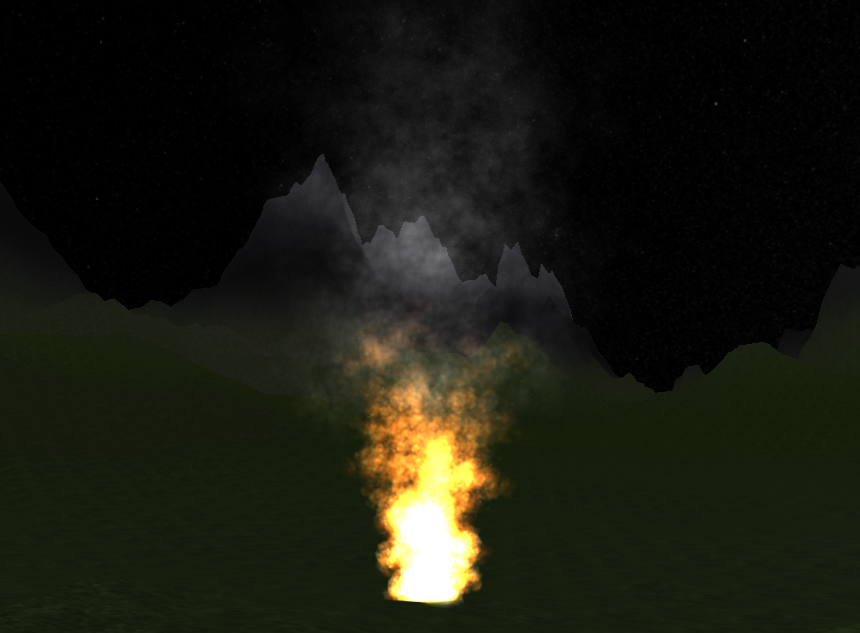
\includegraphics[width=\textwidth]{kepek/particleFinal.png}
% \caption{A végső eredmény hőből fakadó torzítással, és soft particle megvalósítással.}
% \label{fig:particleFinal}
%\end{figure}


\Chapter{Summary}
The main purpose of the thesis was to explore the implementation possibilities of the fire and the related phenomena in computer graphics. I tried to get an insight into the solutions of the problems related to fire rendering through investigation of available game engines, and examined these methods with respect to realism and computational costs. I dealt with real time rendering in the first place, but also investigated some methods that cannot be computed in real time. I tried to implement some of the former ones as well.

I started the investigation with some of the earliest game engines, then moved on to more modern and cmoputationally intense realizations in chronological order. Meanwhile I also gathered some knowledge in the history of the game engines, and learned about some practices to reduce computational costs of the applications, but I did not leave a lot of notes about them. 

I learned about the physical and chemical background of the fire, which helped me to be able to program the phenomenon. I wrote about various methods for rendering fire and made up some ideas to improve realism. Some of these were also successfully implemented by me, which I documented along with some partial and final results.

While working on the thesis I found, that even the smallest details can cause huge problems. Solving these required a lot of research, most of the time I was helped out by documentations, and sometimes I solved problems through dumb luck. While analysing the older game engines I discovered, that you can fight the limitations of the hardware with creativity, although that requires serious skills.

Given the time I was able to implement only as much as I wrote about, but there are still lots of possibilities for improvement. The appereance of the fire could be enhanced using post-processing, and the particles could use some more realistic physics. Attaching light and sound, along with the possibility to interact with fire would be highly benefical for realism.

